\documentclass[french, 11pt]{article} 

%=================================================
% Packages and New Commands
%=================================================

%===== Packages ==================================
%=================================================

\usepackage[utf8]{inputenc}

\usepackage[]{afterpage}
\usepackage[]{amsfonts}
\usepackage[]{amsmath, amssymb}
\usepackage[toc, page]{appendix}
\usepackage[french, english]{babel}
\usepackage[citestyle=verbose-trad2, bibstyle=numeric, sorting=nty]{biblatex}
\usepackage[]{blindtext}
\usepackage[]{booktabs}				% Better tables.
\usepackage[]{caption}
\usepackage[]{chngcntr}
\usepackage[]{csquotes}
\usepackage[]{enumitem}
\usepackage[]{etoolbox}
\usepackage[]{fancyhdr}				% Page headers package.
\usepackage[]{float}
\usepackage[T1]{fontenc}
\usepackage[]{fontspec}
\usepackage[]{gensymb}
\usepackage[a4paper, total={162mm,245mm}, top=28mm]{geometry}
\usepackage[]{graphicx}
\usepackage[]{hyperref}
\usepackage[]{lastpage}
\usepackage[]{layout}
\usepackage[]{listings}				% Code insert package.
\usepackage[]{lmodern}
\usepackage[]{lscape}
\usepackage[]{makecell}
\usepackage[]{mathtools}
\usepackage[]{mathrsfs}
\usepackage[]{mdframed}
\usepackage[]{multicol}
\usepackage[]{multirow}
\usepackage[nottoc]{tocbibind}
\usepackage[]{parskip}
\usepackage[]{pdfpages}
\usepackage[]{pgfplots}
\usepackage[]{soul}
\usepackage[]{subcaption}
\usepackage[]{titlesec}
\usepackage[normalem]{ulem}
\usepackage[]{url}
\usepackage[]{wrapfig}
\usepackage[]{xcolor}

%===== New Commands ==============================
%=================================================

% New command to create a blank page without it being counted on the total page count.
\newcommand{\blankpage}
{
	\null
	\thispagestyle{empty}
	\addtocounter{page}{-1}
	\newpage
}

\newcommand{\question}[1]
{
	\vspace{0.3cm}
	\begin{mdframed}[style=Question]
		#1
	\end{mdframed}
}

\newcommand{\CMDblock}[1]
{
	{\colorbox{black!15}{\texttt{#1}}}
}

\newcommand{\HESSo}{HES$\cdot$So\xspace}
\newcommand{\HESGe}{HES$\cdot$Ge\xspace}

\newcommand{\DocVersion}{1.0.0}

\newcommand{\DocTitle}{Projet Asseto Corsa}
\newcommand{\DocSubject}{Microcontrôleurs et Périphériques}

\newcommand{\SubjectProfessor}{M. Abegg Christian\xspace}

% Make \paragraph as a subsubsubsection
\makeatletter
\renewcommand{\paragraph}{\@startsection{paragraph}{4}{0ex}%
   {-3.25ex plus -1ex minus -0.2ex}%
   {1.5ex plus 0.2ex}%
   {\normalfont\normalsize\bibfont\bf}}
\makeatother

% Make \paragraph appear in TOC
\stepcounter{secnumdepth}
\stepcounter{tocdepth}

%=================================================
% Themes, Colors and Styles
%=================================================

\mdfdefinestyle{Question}{backgroundcolor = black!5, linecolor=black!10, linewidth=2pt}

%=================================================
% Packages Configuration
%=================================================

\hypersetup
{
	bookmarksopen=true,
	pdftitle="\DocTitle\ - \DocSubject",
	pdfauthor="Joachim Bach ; David Da Silva Marques",
	pdfsubject="Bachelor I.S.C",
	pdftoolbar=true,				% Toolbar hidden.
	pdfpagemode=UseOutlines,
	pdfstartview={Fit},				% Fits the width of the page to the window.
	pdfmenubar=true,
	pdfhighlight=/O,
	colorlinks=true,
	pdfpagelayout=OneColumn,
	pdffitwindow=false,
	linktoc=section,
	linkcolor=blue,
	citecolor=blue,
	urlcolor=blue,
}

\bibliography{Others/Bibliography.bib}

\AtEveryCitekey
{
	\clearfield{urldate}
}

%=================================================
% Document Details - Preamble
%=================================================

\title{\DocSubject}
\author{Joachim BACH ; David DA SILVA MARQUES}
\date{\today}

\makeatletter
\let\TheTitle\@title
\let\TheAuthor\@author
\let\TheDate\@date
\makeatother

\pagestyle{fancy}
\fancyhf{}
\lhead{ \textsc{HEPIA Genève} \\ \DocSubject}
\rhead{ \textsc{version} \DocVersion \\ \TheDate}
\cfoot{\thepage \hspace{0.1 mm} / \pageref*{LastPage}}

%=================================================
%=================================================
%=================================================
% Start Document
%=================================================
%=================================================
%=================================================

\begin{document}
	
	\selectlanguage{french}
	\normalsize
	
	\begin{titlepage}
		
		\centering
		\vspace*{2.0 cm}
		
		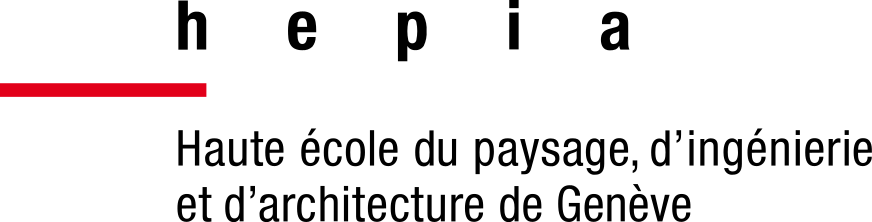
\includegraphics[scale = 1.50]{Images/HEPIA_Logo.png}\\[1.0 cm]
		
		\vspace{1.0 cm}
		
		\rule{\linewidth}{0.3 mm} \\[0.2 cm]
		{\Huge \textbf{\DocTitle}}\\
		\vspace{4 mm}
		{\huge \TheTitle}\\
		\rule{\linewidth}{0.3 mm} \\[1.2 cm]
		
		\textsc{\Large Bachelor I.S.C}\\[0.5 cm]
		
		\vspace{1.5 cm}
		
		\begin{minipage}{0.40\textwidth}
			
			\begin{flushleft}
				\Large\emph{Auteur(s) :}\\[0.2 cm]
				\Large\emph{}\\[0.2 cm]
				\Large\emph{}\\[0.2 cm]
				\Large\emph{}\\[0.2 cm]
				\Large\emph{Institution :}\\[0.2 cm]
				\Large\emph{Date :}\\[0.2 cm]
				\Large\emph{Version :}\\[0.2 cm]
				\Large\emph{Professeur-re :}\\[0.2 cm]
			\end{flushleft}
		
		\end{minipage}~
		\begin{minipage}{0.53\textwidth}
			
			\begin{flushright}
				\Large{Joachim Bach (22650667)}\\[0.2 cm]
				\Large{David Da Silva Marques (226449792)}\\[0.2 cm]
				\Large\emph{}\\[0.2 cm]
				\Large{HEPIA Genève}\\[0.2 cm]
				\Large{\TheDate}\\[0.2 cm]
				\Large{\DocVersion}\\[0.2 cm]
				\Large{\SubjectProfessor}\\[0.2 cm]
			\end{flushright}
		
		\end{minipage}
	
	\end{titlepage}
	
	\blankpage

    \section{Introduction}

    Dans le cadre du cours Microcontrôleur et Périphériques (MIPS), nous avons dû réaliser un projet. Celui-ci a pour but, et exigences, de réunir l'ensemble des interfaces et fonctionnalités étudiées durant ce semestre.

    La contrainte principale est que nous devions utiliser deux cartes MyLab2. Nous avions aussi pour obligation d'utiliser les interfaces suivantes :

    \begin{enumerate}
        \item CAN
        \item Écran avec texte
        \item Communication UART
        \item Dalle tactile
        \item SysTick / Timer
        \item Boutons
    \end{enumerate}

    \subsection{Présentation du projet}

    Le projet que nous avons choisi consiste à développer une sorte de manette de jeu pour jouer au simulateur de course automobile "Assetto Corsa". 
	
	Voici une description de l'utilisation des deux MyLab2 : 
	Une des deux cartes sert de volant, grâce à l'accéléromètre, avec des boutons pour l'accélérateur et le frein. Les LEDS du dipswitchs sont utilisées comme indicateur de compte-tours. L'autre carte sert de tableau de bord affichant la télémétrie du jeu et ayant un ensemble de boutons pour permettre quelques inputs supplémentaires.

	% //TODO add final physical image of the setup

    \section{Architecture}

		Dans cette section de notre rapport, nous allons présenter les différentes parties composant notre périphérique. Il s'agira de discuter de la partie PC, de la carte servant de volant ainsi que de celle servant de tableau de bord.

		\subsection{Schéma de l'architecture}

			Voici un schéma conceptuel décrivant l'architecture mise en place dans le cours de ce travail pratique :

			\begin{figure}[H]
				\centering
				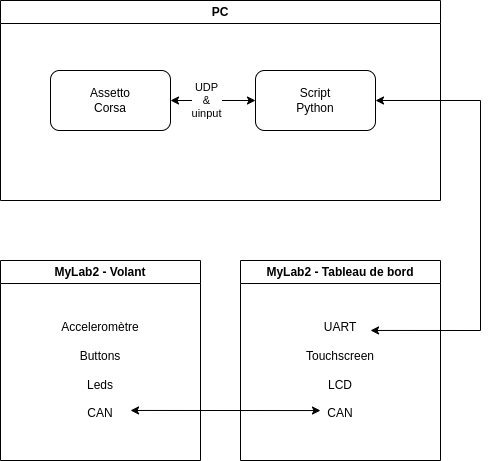
\includegraphics[width=0.55\textwidth]{Images/architecture.drawio.png}
				\caption{Schéma de l'architecture}
			\end{figure}
			
        \subsection{Implémentation côté PC}

        Du côté du PC se trouve Assetto Corsa, un jeu de voiture ainsi qu'un script python tournant en arrière-plan. Ce script python se charge de récupérer la télémétrie d'Assetto Corsa à travers un socket UDP mis à disposition par le jeu (il s'agit d'une méthode d'accès à la télémétrie courante dans le monde des simulateurs). Le python récupère alors les informations qui l'intéressent et les envoie sur l'UART vers le "Tableau de bord", autrement dit l'une des deux cartes. 
		
		Depuis cette même connexion UART, le script récupère les inputs (inclinaison du volant, pression des boutons, etc.) sous forme de tableau d'octets envoyé par la carte tableau de bord. Ces informations sont ensuite transmises à une classe "Gamepad" qui simule un périphérique qui est ensuite utilisée par le jeu comme un n'importe quel autre périphérique/manette/etc et qui est ainsi utilisable en jeu.

		% //TODO mettre une image du jeu avec le script qui toure à côté


        \subsection{MyLab2 Volant}

		La carte MyLab2 servant de volant est celle tenue entre les mains du joueur. Son rôle est de simuler un volant de course et doit ainsi permettre de guider la voiture, mais aussi de contrôler l'accélérateur, les freins et d'afficher quelques informations sur la voiture.

        Le volant s'occupe alors de récupérer les valeurs de son accéléromètre et de les convertir en un angle. Il envoie en continu le résultat de ce calcul par CAN à a carte servant de tableau de bord. Lors de l'appui sur le bouton A ou B, un message CAN est transmis immédiatement au tableau de bord. 
		
		Le volant reçoit sur le CAN, les RPM du moteur et la vitesse de la voiture. Ceux-ci seront affichés respectivement sur les LEDS des dipswitchs et sur le LCD sous forme de cadrant avec une aiguille.

		% //TODO mettre une image de près du volant
        
        \subsection{MyLab2 Tableau de bord}

        Le tableau de bord est la pièce centrale du projet : cette carte sert d'intermédiaire entre le volant et le PC. Le tableau de bord reçoit à travers l'UART la télémétrie venant du jeu, dont il affiche l'accélérateur et le frein, mais aussi le temps du tour (lap time). Il retransmet ensuite la vitesse et les RPM au volant via CAN. De celui-ci il récupère la rotation et les boutons, qu'il stocke dans un tableau local. Toutes les 20ms, il envoie alors ce tableau par la même connexion UART pour que le PC puisse interpréter les inputs. 

        \subsection{Matériel}    

        Pour ce projet nous avons donc besoin :

        \begin{enumerate}
            \item 1 PC avec Assetto Corsa et 1 script python permettant d'interfacer avec les cartes
            \item 2 MyLab2 + LPC1769
            \item 1 câble USB A → micro-USB
            \item 1 câble CAN
            \item Câbles d'alimentation
        \end{enumerate}


	\section{Problèmes rencontrés}

	Initialement il avait été prévu que les cartes soient utilisé en tant périphériques USB. Cependant, il s'avère que c'est un protocole relativement sensible et précis, rendant compliqué son implémentation dans un délai aussi court. Heureusement un plan de secours avait été prévu, utiliser un script python couplé à de l'UART pour la transmission des données pour pouvoir simuler un périphérique logiciellement. Cependant, cette solution n'est pas miraculeuse et ne fonctionne pas de manière stable.

    \section{Conclusion}



\end{document}